% !TeX root = ../main.tex

\chapter{Device evaluation and dispersion analysis}% from transmission spectroscopy

%\section{Methods}

In the example given in \autoref{sec:disp-comp},  a typical dispersive ring resonator has the $ D_2 $ value less than MHz, which means the frequency FSR, for example 100 GHz, is different from the next one with a MHz-level difference. 
It is difficult to achieve such precise measurement using traditional optical spectrum analyzer whose typical resolution is around pm, 100 MHz. The tunable laser scanning is developed to solve this problem, especially assisted by an external frequency comb \cite{Liu2016d}. 

Here, we exploit the method using laser step triggering to calibrate the real-time measured device transmission.


\section{Setups}

In previous works \cite{Sunada2018}, both grating coupling and edge coupling were studied. In this research, considering the broadband frequency conversion motivation, the edge coupling is preferred due to the broader 3 dB bandwidth. Aligned with the lensed fiber at two five-axis fiber alignment stages (Newport M-562F-XYZ \& M-562F-XYZ-LH), the best facet-to-facet coupling efficiency around 6 dB is achieved using the lensed fibers with a spot size of 2 \si{\um}.
A more typical facet-to-facet loss of LS-CVD samples can be 8-9 dB.
It is worth mentioning that a chip arrier (SURUGA SEIKI F126) equipped with a thermoelectric cooler (TEC) is used on the device stage, which is essential for long-time thermal stability. To prevent moisture condensation, the TEC is set a little bit higher than room temperature, 30 \si{\celsius} in our case. 


\begin{figure}
	\centering
	\includesvg[width=.9\textwidth]{trans_setup}
%	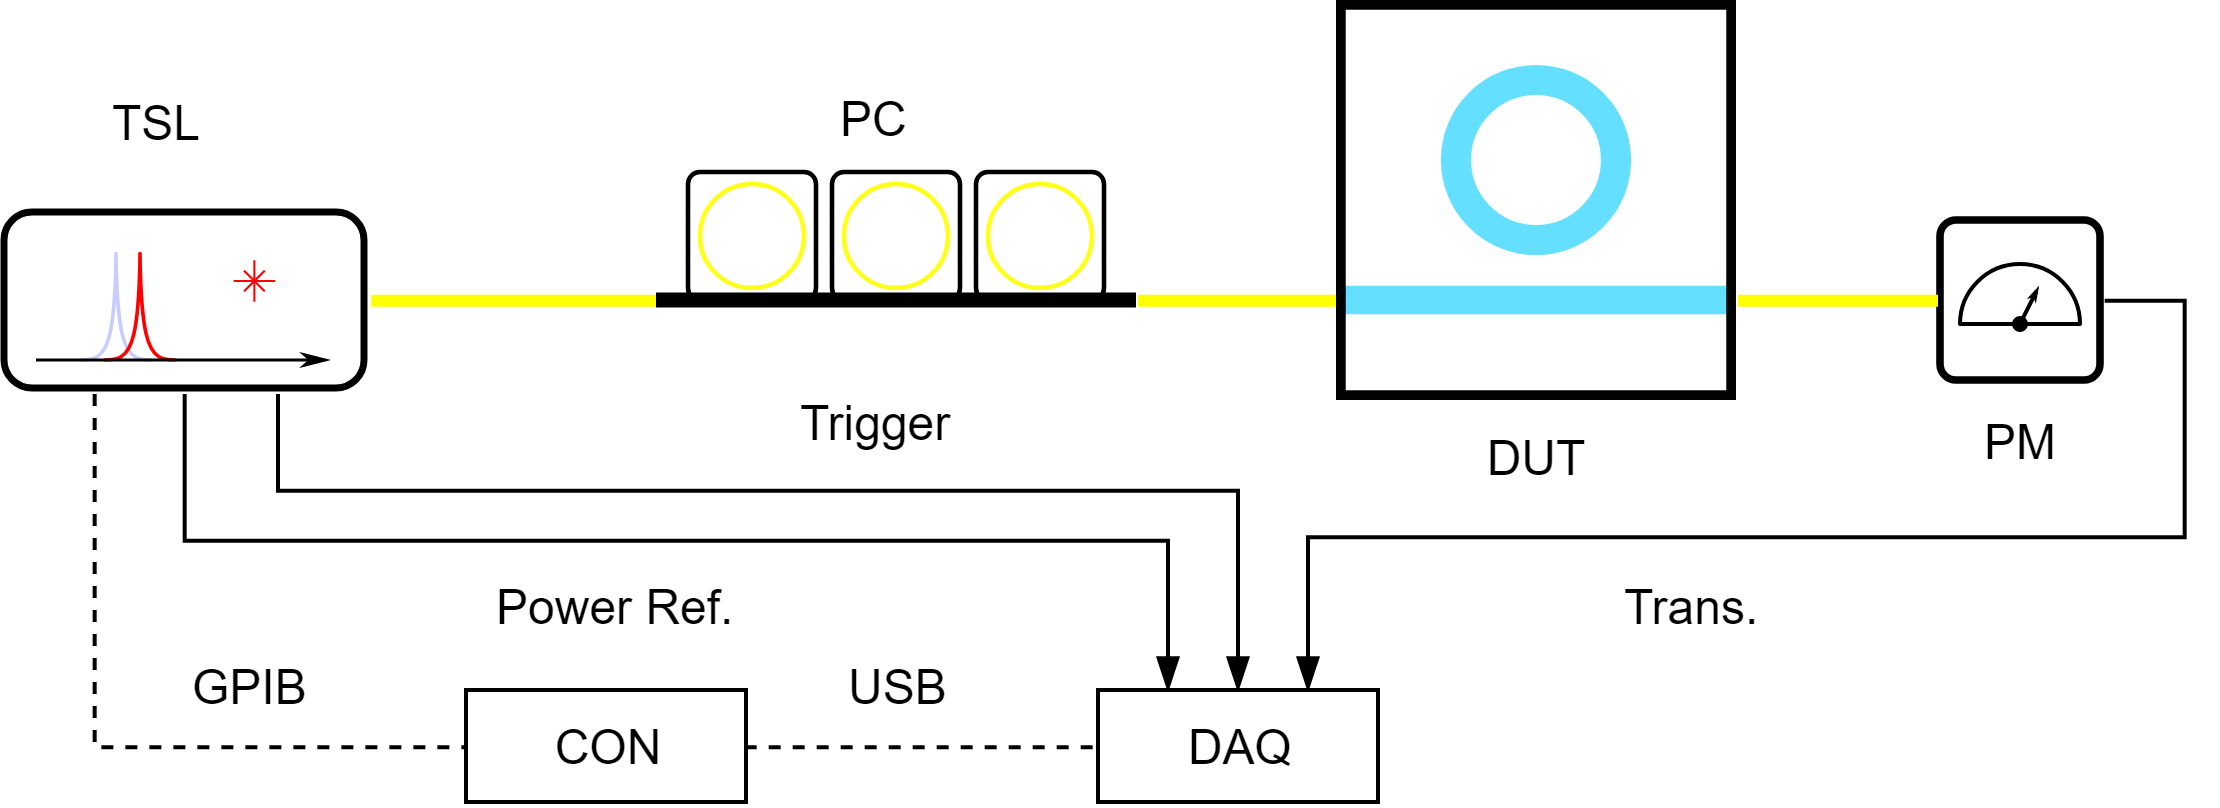
\includegraphics[width=.9\textwidth]{imgs/png/trans_setup}
	\mycaption{Setup of transmission measurement system}{TSL, tunable semiconductor laser. PC, optical fiber polarization controller. DUT, device under test. PM, power meter. DAQ, data acquisition.}
	\label{fig:transsetup}
\end{figure}

The schematic diagram of the device spectrum measurement is shown in \autoref{fig:transsetup}. Before the spectrum scanning, the output port is coupled to the infrared InGaAs camera in free space using a 20$\times$ objective lens. By carefully rotating the palette of polarization controller on the input side, the device can be launched in either TE or TM mode. Next, the TSL (SANTEC TSL-710) is set to sweep from 1480 nm - 1640 nm, covering the telecom S C and L bands. The internal power reference signal and the step trigger are also generated simultaneously. Compared with photon diodes, the power meter (Newport 2963-R) in our setup is critical to realize the scanning at various power ranges.  Finally, the signals from power monitor, step trigger and device transmission are all collected with the same data acquisition module, and then analyzed by the computer.
% \section{Results}

\section{Results}

\subsection{Thermal stability}

\begin{figure}
	\centering
	\includesvg[width=1\textwidth]{thermal}
	%	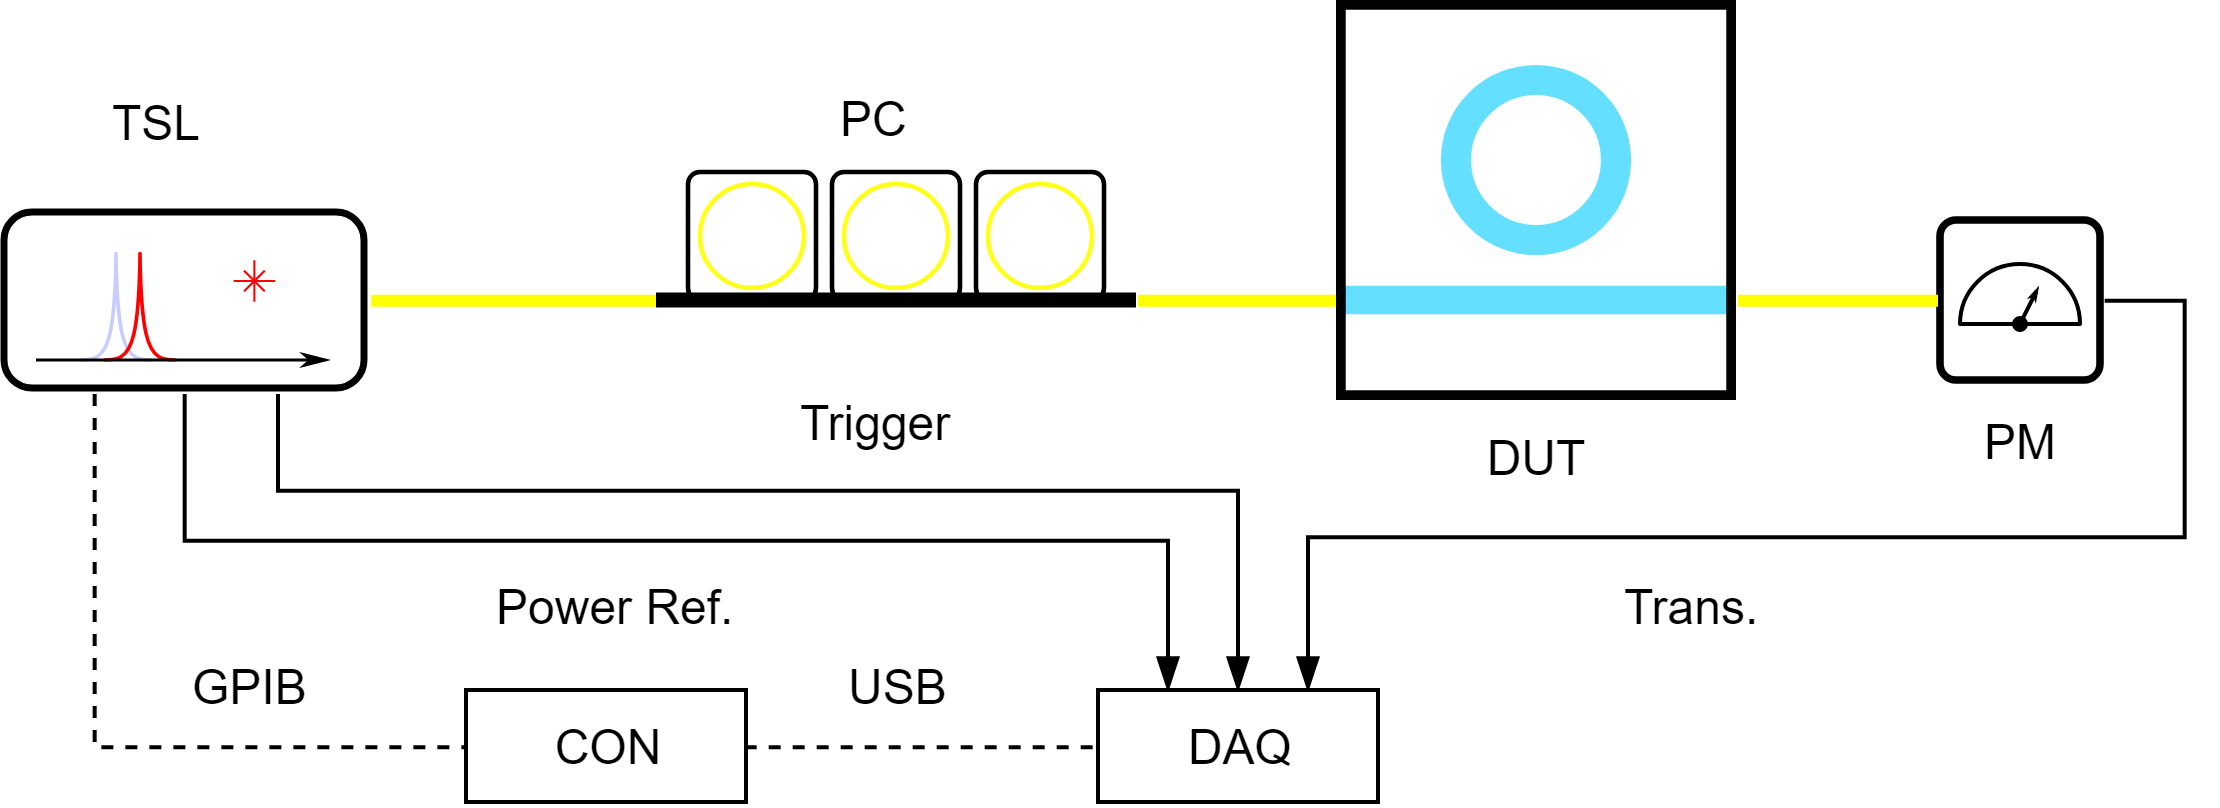
\includegraphics[width=.9\textwidth]{imgs/png/trans_setup}
	\mycaption{}{}
	\label{fig:thermal}
\end{figure}

%\begin{figure}
%	\centering
%	\includesvg[width=.9\textwidth]{dwldT}
%	%	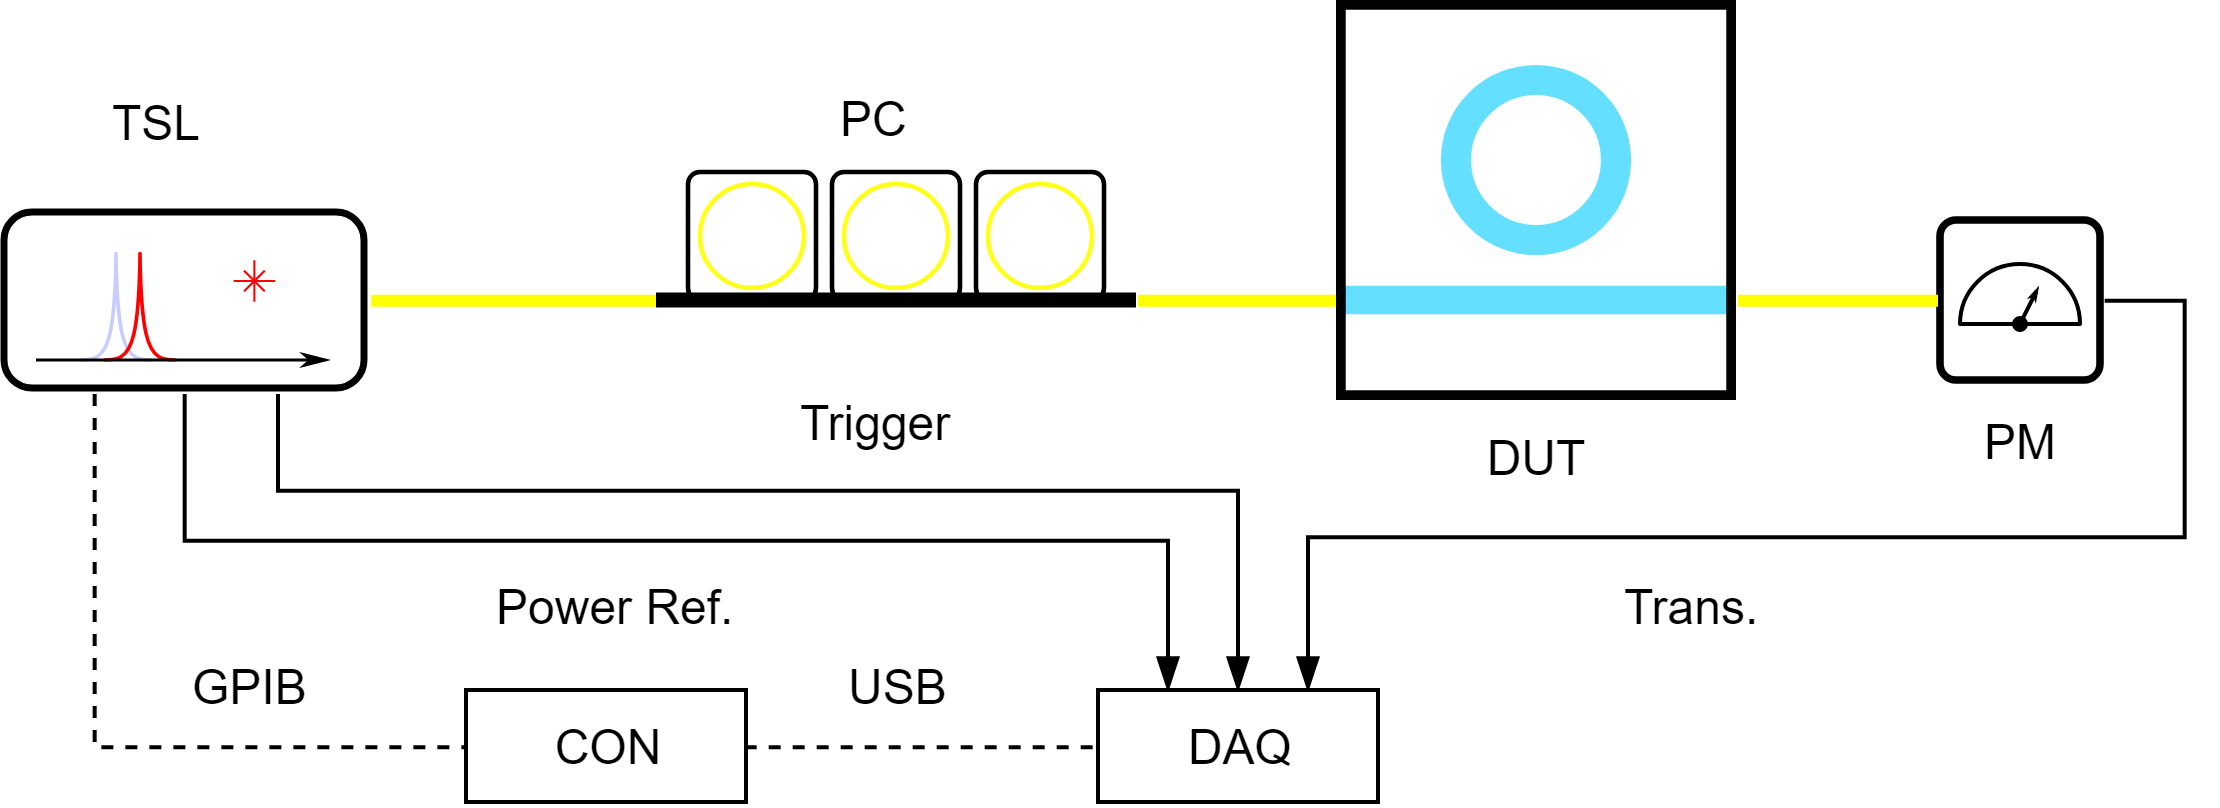
\includegraphics[width=.9\textwidth]{imgs/png/trans_setup}
%	\mycaption{}{}
%	\label{fig:wl-T}
%\end{figure}

Although silicon nitride is reported as high thermal conductivity material, the surrounding silicon dioxide is comparatively bad thermal-conductive. Since the nonlinear phenomena usually requires high pump power, which heats the device significantly, the thermal stability is thus a critical factor of nonlinear ring resonators.

With the TEC tuned into different temperatures, the normalized transmission then measured, giving the thermal dependence of resonant wavelength. The transmission is shown in \autoref{fig:thermal}a and the extracted resonant wavelengths are plotted in \autoref{fig:thermal}b.

\subsection{Device transmission}

\subsection{Dispersion analysis}
